%%%%%%%%%%%%%%%%%%%%%%%%%%%%%%%%%%%%%%%%%
% Beamer Presentation
% LaTeX Template
% Version 1.0 (10/11/12)
%
% This template has been downloaded from:
% http://www.LaTeXTemplates.com
%
% License:
% CC BY-NC-SA 3.0 (http://creativecommons.org/licenses/by-nc-sa/3.0/)
%
%%%%%%%%%%%%%%%%%%%%%%%%%%%%%%%%%%%%%%%%%

%----------------------------------------------------------------------------------------
%	PACKAGES AND THEMES
%----------------------------------------------------------------------------------------

\documentclass{beamer}

\mode<presentation> {

% The Beamer class comes with a number of default slide themes
% which change the colors and layouts of slides. Below this is a list
% of all the themes, uncomment each in turn to see what they look like.

%\usetheme{default}
%\usetheme{AnnArbor}
%\usetheme{Antibes}
%\usetheme{Bergen}
%\usetheme{Berkeley}
%\usetheme{Berlin}
%\usetheme{Boadilla}
%\usetheme{CambridgeUS}
%\usetheme{Copenhagen}
%\usetheme{Darmstadt}
%\usetheme{Dresden}
%\usetheme{Frankfurt}
%\usetheme{Goettingen}
%\usetheme{Hannover}
%\usetheme{Ilmenau}
%\usetheme{JuanLesPins}
%\usetheme{Luebeck}
%\usetheme{Madrid}
%\usetheme{Malmoe}
%\usetheme{Marburg}
%\usetheme{Montpellier}
\usetheme{PaloAlto}
%\usetheme{Pittsburgh}
%\usetheme{Rochester}
%\usetheme{Singapore}
%\usetheme{Szeged}
%\usetheme{Warsaw}

% As well as themes, the Beamer class has a number of color themes
% for any slide theme. Uncomment each of these in turn to see how it
% changes the colors of your current slide theme.

%\usecolortheme{albatross}
%\usecolortheme{beaver}
%\usecolortheme{beetle}
%\usecolortheme{crane}
%\usecolortheme{dolphin}
%\usecolortheme{dove}
%\usecolortheme{fly}
%\usecolortheme{lily}
%\usecolortheme{orchid}
%\usecolortheme{rose}
%\usecolortheme{seagull}
%\usecolortheme{seahorse}
%\usecolortheme{whale}
%\usecolortheme{wolverine}

%\setbeamertemplate{footline} % To remove the footer line in all slides uncomment this line
%\setbeamertemplate{footline}[page number] % To replace the footer line in all slides with a simple slide count uncomment this line

%\setbeamertemplate{navigation symbols}{} % To remove the navigation symbols from the bottom of all slides uncomment this line
}

\usepackage{graphicx} % Allows including images
\usepackage{booktabs} % Allows the use of \toprule, \midrule and \bottomrule in tables
\usepackage{multimedia}
\usepackage{hyperref}

%----------------------------------------------------------------------------------------
%	TITLE PAGE
%----------------------------------------------------------------------------------------

\title[FlappyPi]{The Summer C Project and FlappyPi} % The short title appears at the bottom of every slide, the full title is only on the title page

\author[Group 16]{\small Henryk~Haddass \and Mickey~Li \and Michael~Radigan \and Oliver~Wheeler}% Your name
\institute[Imperial DoC] % Your institution as it will appear on the bottom of every slide, may be shorthand to save space
{
Group 16
\medskip
}
\date{\today} % Date, can be changed to a custom date

\begin{document}

\begin{frame}
\titlepage % Print the title page as the first slide
\end{frame}

\begin{frame}
\frametitle{Overview} % Table of contents slide, comment this block out to remove it
\tableofcontents % Throughout your presentation, if you choose to use \section{} and \subsection{} commands, these will automatically be printed on this slide as an overview of your presentation
\end{frame}

%----------------------------------------------------------------------------------------
%	PRESENTATION SLIDES
%----------------------------------------------------------------------------------------

%------------------------------------------------
\section{Emulator} % Sections can be created in order to organize your presentation into discrete blocks, all sections and subsections are automatically printed in the table of contents as an overview of the talk

%------------------------------------------------

\subsection{Implementation} % A subsection can be created just before a set of slides with a common theme to further break down your presentation into chunks

\begin{frame}
\frametitle{}






\end{frame}

%------------------------------------------------
\subsection{Outcome}
\begin{frame}
\frametitle{Bullet Points}




\end{frame}

%------------------------------------------------
\subsection{Evaluation}


\begin{frame}
\frametitle{Problems and Challenges}


\begin{block}{Block 1}
Lorem ipsum dolor sit amet, consectetur adipiscing elit. Integer lectus nisl, ultricies in feugiat rutrum, porttitor sit amet augue. Aliquam ut tortor mauris. Sed volutpat ante purus, quis accumsan dolor.
\end{block}

\begin{block}{Block 2}
Pellentesque sed tellus purus. Class aptent taciti sociosqu ad litora torquent per conubia nostra, per inceptos himenaeos. Vestibulum quis magna at risus dictum tempor eu vitae velit.
\end{block}

\begin{block}{Block 3}
Suspendisse tincidunt sagittis gravida. Curabitur condimentum, enim sed venenatis rutrum, ipsum neque consectetur orci, sed blandit justo nisi ac lacus.
\end{block}



\end{frame}

%------------------------------------------------

\begin{frame}
\frametitle{Improvements}
%\frametitle{Multiple Columns}
\begin{columns}[t] % The "c" option specifies centered vertical alignment while the "t" option is used for top vertical alignment

\column{.5\textwidth} % Left column and width
\begin{itemize}
\item Statement
\item Explanation
\item Example
\end{itemize}



\column{.5\textwidth} % Right column and width
\begin{itemize}
\item Statement
\item Explanation
\item Example
\end{itemize}

\end{columns}
\end{frame}


%------------------------------------------------
\section{Assembler}
%------------------------------------------------


\subsection{Implementation}

\begin{frame}
\frametitle{Our Approach}

We used a simple 3 modules approach - \textit{assemble.c}, \textit{dictionary.c} and \textit{encode.c}. 
\\~\\

Characteristics of our assembler include: 
\begin{itemize}
\item 2 pass assembler method

\item Polymorphic AVL Tree ADT dictionary

\item Using the Dictionary to map functions to Opcodes

\item Each Function decodes the instruction string themselves

\end{itemize}

\end{frame}

%------------------------------------------------

\begin{frame}
\frametitle{Structure}

\begin{figure}[c]
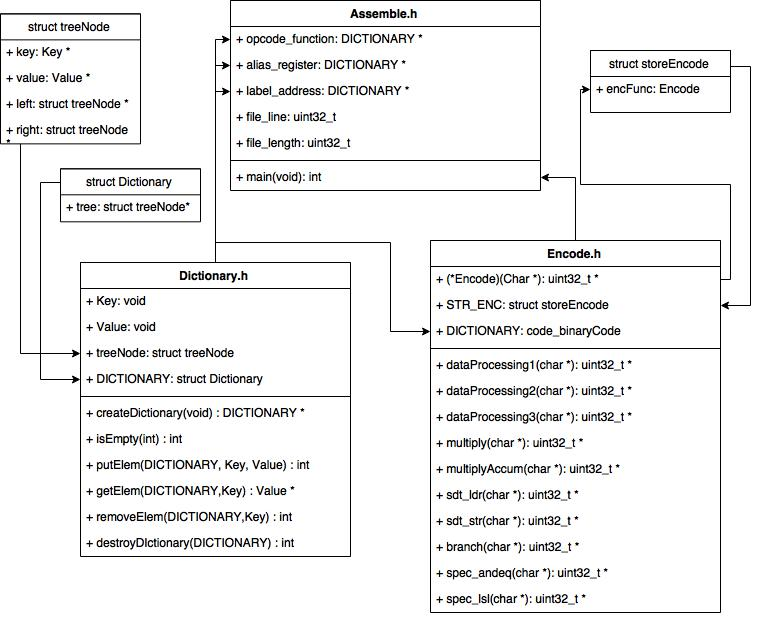
\includegraphics[width=0.9\linewidth]{Images/Assembler_XML.jpg}
\end{figure}


\end{frame}

%------------------------------------------------
\subsection{Outcome}
\begin{frame}[fragile] % Need to use the fragile option when verbatim is used in the slide 
\frametitle{Outcome - Disassembler}

\begin{figure}
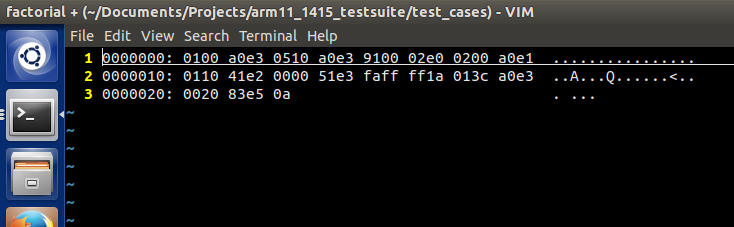
\includegraphics[width=1\linewidth]{Images/Screen1.png}
\end{figure}

\begin{figure}
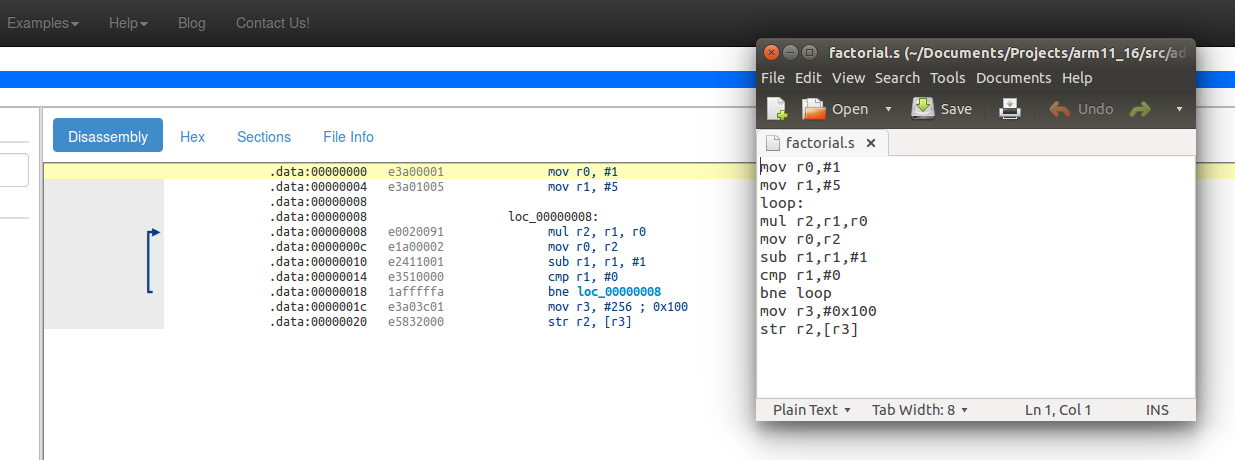
\includegraphics[width=1\linewidth]{Images/Screen2.png}
\end{figure}

\end{frame}

%------------------------------------------------
\subsection{Evaluation}
\begin{frame}
\frametitle{Problems and Challenges}
\begin{description}
\item[String Tokenising]\hfill\\
	Using \textbf{strtok()} and \textbf{sscanf()} proved to be very limiting
	
\item[Dictionary ADT]\hfill\\
	Development of the AVL tree was time consuming and took a long time before it was bug free
	
\item[Memory Allocation]\hfill\\
	Many mistakes and errors ended up being A problem with the use of \textbf{malloc()} and \textbf{free()}.

\item[Code Reuse]\hfill\\
	The compactness of the \textit{Emulator} code meant it was difficult to reuse within assembler. 


\end{description}
\end{frame}

%------------------------------------------------

\begin{frame}
\frametitle{Improvements}
\begin{itemize}
	\item Creating our own string tokeniser which is more flexible then the implementation of \textbf{strtok()}.
	\item Spending a bit more time optimising and improving the quality of the code.
	\item 
\end{itemize}
\end{frame}

%------------------------------------------------
\section{Proof of use}
%------------------------------------------------
\begin{frame}
\frametitle{Flashing GPIO}

\begin{figure}
%\movie[width=3cm,height=2cm,poster]{}{Testvideo.mp4}
%\movie[width=3cm,height=2cm,poster]{}{test1.mpg}

\movie[label=cells,width=4cm,height=3cm,poster,showcontrols,duration=5s]{}{test1.mpg}
\hyperlinkmovie[start=5s,duration=7s]{cells}{\beamerbutton{Show the middle stage}}
\hyperlinkmovie[start=12s,duration=5s]{cells}{\beamerbutton{Show the late stage}}

\caption{Our Flashing Gpio Led}
\end{figure}


\end{frame}
%------------------------------------------------
\section{Extension}
%------------------------------------------------

\subsection{Implementation}

\begin{frame}
\frametitle{FlappyPi}





\end{frame}

%------------------------------------------------
\begin{frame}
\frametitle{Extending the Assembler}
To make it possible for us to use our own Assembler to process the assemble source code, we have had to do the following:
\\~\\
\begin{description}
\item[Stack (block data transfer)]\hfill\\
	Enabling the use of \textbf{stm} and \textbf{ldm} in the assembler, so that the stack can be utilised.
	
\item[Opcodes Suffixes]
	Supporting the addition of the 2 character condition codes on the end of the existing opcodes

\item[Aliasing]
	

\item[Multi-File Programs]


\end{description}
\end{frame}
%------------------------------------------------
\subsection{Outcome}

\begin{frame}
\frametitle{Problems and Challenges}





\end{frame}


%------------------------------------------------
\subsection{Evaluation}

\begin{frame}
\frametitle{Improvements}





\end{frame}


%-------------------------------------------------
\section{Project Evaluation}
%-------------------------------------------------
\subsection{Evaluation}
\begin{frame}

\frametitle{Problems and Challenges}

\begin{description}

\item[Organisation]\hfill\\
	\begin{itemize}
	\item Lack of a Complete Plan from the start
	\item Redundant code
	\item Regularly missed personal deadlines
	\item Distribution of tasks
	\end{itemize}

\item[Communication]\hfill\\
	\begin{itemize}
	\item Instant messenger issues
	\item Lack of Clarity
	\item Sleeping Pattens
	\end{itemize}

\item[Effectiveness]\hfill\\
	\begin{itemize}
	\item C knowledge
	\item Testing and Debugging
	\item Git
	\end{itemize}


\end{description}




\end{frame}
%-------------------------------------------------
\begin{frame}

\frametitle{Use of GIT}





\end{frame}


%-------------------------------------------------
\subsection{Improvements}
\begin{frame}

\frametitle{Improvements}





\end{frame}

%-------------------------------------------------
\begin{frame}

\frametitle{Conclusion}





\end{frame}


\end{document} 